\chapter{Разработка приложения для генерации нормализованных систем уравнений} \label{ch2}
	
\section{Общие сведения} \label{ch2:intro}

Приложение имеет консольный интерфейс на английском языке. Сгенерированные данные записываются в файлы (подробнее описано ниже). При запуске приложения можно ввести ключ \(/h\) для вызова справки или задать аргументы. Аргументы должны вводиться в следующем порядке:
\begin{enumerate}
	\item Первый – количество уравнений в генерируемой системе (натуральное число). Обязателен.
	\item Второй аргумент, если задан – ключ запуска. Допускаются ключи:
	\begin{enumerate}
		\item \(/s\) –- тихий запуск, в этом режиме в папку записываются только файлы с системой, её решением и нормализованной системой;
		\item \(/r\) –- стандартный запуск (по умолчанию), в этом режиме в папку записываются те же файлы, что в тихом режиме, а также исходные данные и все промежуточные результаты;
		\item \(/t\) –- запуск в режиме тестирования, в этом случае осуществляется стандартный запуск, после чего происходит тестирование для различных векторов. Процесс тестирования описан ниже.
	\end{enumerate} 
	\item Третий аргумент, если задан –- имя папки, куда будут записаны сгенерированные файлы. Если директория с таким именем не существует, она будет предварительно создана. По умолчанию используется имя “results”.
\end{enumerate} 

В папке, имя которой передается третьим аргументом, создается папка с именем вида YYYY.MM.DD\_HH.MM.SS –- определяется системной датой и временем. В эту папку записываются сгенерированные данные в следующих файлах:
\begin{enumerate}
	\item Случайно сгенерированные исходные данные:
	\begin{enumerate}
		\item pre\_rand/M1.txt – матрица \(M_1\);
		\item pre\_rand/M2.txt – матрица \(M_2\);
		\item pre\_rand/v1.txt – вектор \(v_1\);
		\item pre\_rand/v2.txt – вектор \(v_2\).
	\end{enumerate} 
	\item Промежуточные данные:
	\begin{enumerate}
		\item pre\_gen/S.txt – преобразование \(S\);
		\item pre\_gen/T.txt – преобразование \(T\);
		\item pre\_gen/F.txt – преобразование \(F\);
		\item inv/invM1.txt – матрица, обратная к  \(M_1\);
		\item inv/invM2.txt – матрица, обратная к  \(M_2\);
		\item inv/invF.txt – преобразование, обратное к  \(F\);
	\end{enumerate} 
	\item Результат работы программы:
	\begin{enumerate}
		\item P.txt – ненормализованная система уравнений;		\item P\_sol.txt – решение ненормализованной системы уравнений;
		\item P\_norm.txt – нормализованная система уравнений;
	\end{enumerate} 
\end{enumerate} 



%%%%
%%		
%%  \input{...} commands are used only to sychronize some parts of the text with the author guide. Authors are free to type the text directly in .tex-files   
%%  \input{...} комманды используются только, чтобы синхронизировать части текта с рекомендациями авторам. Авторы  вольны вносить текст непосредственно в файл главы  
%%  
% %% ВНИМАНИЕ: для того, чтобы избежать лишнего отступа между текстом  и формулами, пожалуйста, начинайте формулы без пропуска строки в исходном коде как в строках #2 и #3.
	Все формулы, размещенные в отдельных строках, подлежат нумерации, например, как формулы \eqref{eq:UpArrow-G} и \eqref{eq:DownArrow-G} из \cite{Ganter1999}. 
	\begin{align}
	\label{eq:UpArrow-G}
	& A\uA =  \{ m\in{}M\:|\:gIm\:\forall  g \in{} A \}; \\ 
	\label{eq:DownArrow-G}
	& B\dA =  \{ g\in{}G\:|\:gIm\:\forall  m \in{} B \}.
	\end{align}

Обратим внимание, что формулы содержат знаки препинания и что они выровнены по левому краю (с помощью знака \verb|&| окружения \texttt{align}). % пример двух выравнивания двух формул в окружении align


%На \firef{fig:spbpu-new-bld-autumn-ch2} приведёна фотография Нового научно-исследовательского корпуса СПбПУ.

%	\begin{figure}[ht] 
%	\center
%	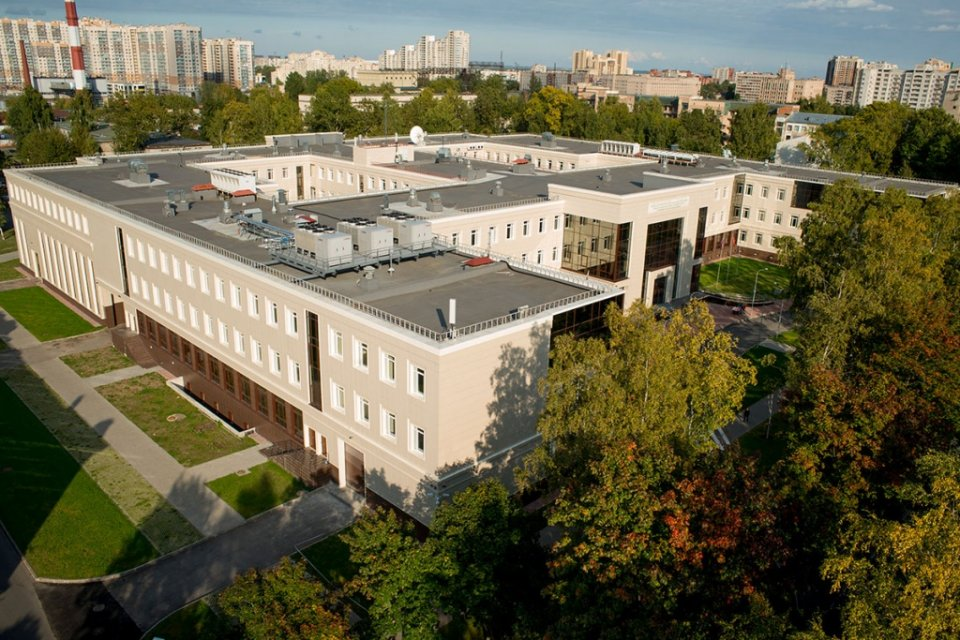
\includegraphics [scale=0.27] {my_folder/images/spbpu_new_bld_autumn}
%	\caption{Новый научно-исследовательский корпус СПбПУ \cite{spbpu-gallery}} 
%	\label{fig:spbpu-new-bld-autumn-ch2}  
%	\end{figure}
	
\section{Детали реализации} \label{ch2:sec-abbr} %название по-русски
	
Наиболее важные элементы реализации приложения описаны далее в этом разделе. 	

\subsection{Служебные модули} \label{ch2:subsec-title-abbr} %название по-русски

Реализация базируется на следующих служебных модулях:
\begin{enumerate}
	\item \(Utility\) -- содержит используемые в других модулях строковые функции.
	\item \(File\_system\) -- содержит функции, используемые при работе с файловой системой.
	\item \(BOOL\) -- псевдоним для типа данных \(int\), также определены константы  \(FALSE = 0\)  и  \(TRUE = 1\).  Он используется в качестве замены логического типа данных, что позволяет достичь увеличения скорости работы с данными на 30-50\%.
\end{enumerate} 

			
\subsection{Матрицы} \label{ch2:subsec-title-abbr} %название по-русски

В пространстве имен \(matrixes\) описаны следующие классы:
\begin{enumerate}
	\item \(Row\) -- описывает строку матрицы или вектор-столбец. Агрегирует объект типа \(std::vector<BOOL>\).
	\item \(Matrix\) -- описывает квадратную матрицу, агрегирует объект типа \(std::vector<Row<BOOL> *>\). Использование указателей позволяет заметно снизить накладные расходы. Реализован метод \(init\_zeros()\), который задает размерность матрицы и инициализирует ее нулями, и метод \(initInverse()\), инициализирующий матрицу как матрицу, обратную по отношению к переданной по ссылке в качестве параметра.
	\item \(MatrixBuilder\) -- реализует паттерн Строитель, предоставляет удобный интерфейс для определения объектов \(Matrix\).
\end{enumerate} 


\subsection{Полиномы} \label{ch2:subsec-title-abbr} %название по-русски

В пространстве имен \(polynomials\) описаны следующие классы:
\begin{enumerate}
	\item \(Monomial\) -- представляет моном, или же терм. Так как все конструкции находятся в поле \(GF(2)\), степени всех переменных не превышают первую, поэтому хранится только список переменных, представленных в терме (в виде вектора). Так как полиномы генерируются самим приложением, становится возможной дальнейшая оптимизация: хранить только номера переменных, а их названия определять простым добавлением номера к букве х. Так, переменная x5 имеет номер 5. Все коэффициенты также равны единице, поэтому тоже не хранятся. Основные методы –- \(simplify()\), вызываемый после каждого изменения структуры терма, в том числе в конце работы конструктора, он гарантирует упорядоченность переменных по возрастанию; и метод \(substitute()\), подставляющий набор значений переменных в моном и возвращающий результат типа \(BOOL\).
	\item \(Polynomial\) -- описывает полином, представляет собой вектор мономов. Определены операторы \(+=\) и \(*=\), позволяющие прибавлять моном и домножать на моном, соответственно. Определен метод \(substitute()\), рекурсивно вызывающий метод \(substitute()\) каждого монома. Мономы в каждый момент отсортированы, за что отвечает метод \(simplify()\). Порядок сортировки следующий:
	\begin{enumerate}
		\item Мономы большей степени расположены раньше, чем мономы меньшей степени;
		\item Мономы равной степени сортируются лексикографически.
	\end{enumerate} 
	\item Также в пространстве имен \(polynomials\) определены классы, реализующие паттерн Строитель: \(MonomialBuilder\), упрощающий создание объектов \(Monomial\), и \(PolynomialBuilder\) и \(DNFBuiler\) – они оба упрощают создание объектов \(Polynomial\), но по-разному: \(PolynomialBuilder\) собирает полином из мономов, а \(DNFBuilder\) собирает полином как сумму других полиномов.
\end{enumerate} 


\subsection{Генерация псевдослучайных объектов} \label{ch2:subsec-title-abbr} %название по-русски

Генерация псевдослучайных объектов (ПСО) не может обеспечиваться независимым вызовом функции-генератора псевдослучайных чисел (ГПСЧ), так как вызовы могут поступать с интервалом менее одной секунды, в результате чего различные объекты будут инициализироваться одинаковыми значениями. В связи с этим создано пространство имен \(random\), содержащее несколько классов. Они генерируют случайные объекты, используя один и тот же объект ГПСЧ:
\begin{enumerate}
	\item \(RandomEngine\) -- хранит ГПСЧ \(std::mt19937\) (вихрь Мерсенна). Имеет метод \(getRandomEngine()\), возвращающий константную ссылку на этот объект. Используется для инициализации ГПСЧ других классов этого пространства имен.
	\item \(RandomMatrixFactory\) -- реализует паттерн Фабрика, генерирует ПСО типа \(Matrix\) и \(Row\).
	\item \(RandomPolynomialFactory\) -- реализует паттерн Фабрика, генерирует ПСО типа \(Polynomial\) (полином второй степени).
\end{enumerate} 


\subsection{Преобразования} \label{ch2:subsec-title-abbr} %название по-русски

В пространстве имен \(transformations\) определены следующие классы:
\begin{enumerate}
	\item \(Transformation\) –- определяет преобразование. Инкапсулирует \(std::vector<Polynomial>\), каждый полином соответствует преобразованию одной координаты. В нем определен метод \(initComposition()\), инициализирующий преобразование как композицию двух преобразований, передаваемых по константной ссылке. Также определен метод \(substitute()\), вызывающий метод \(substitute()\) для полиномов всех координат, и возвращающий \(std::vector<BOOL>\) (по ссылке, чтобы избежать лишнего копирования), и метод \(normalize()\), нормализующий систему (алгоритм его работы представлен в соответствующем разделе ниже).
	\item \(AffineTransformation\) –- наследуется от класса \(Transformation\) и позволяет определять аффинное преобразование по матрице \(M\) и вектору \(v\) как \(F(x) = Mx + v\).
	\item \(TransformationBuilder\) –- реализует паттерн строитель для объектов \(Transformation\).
\end{enumerate} 


\subsection{Ввод-вывод} \label{ch2:subsec-title-abbr} %название по-русски

Для организации единообразной структуры ввода-вывода в проекте в пространстве имен \(IO\) определены следующие классы:
\begin{enumerate}
	\item \(Writer\) –- производит запись в файл, инкапсулирует объект типа \(ofstream\). Может записывать в файл объекты типов \(Row\), \(Matrix\), \(Polynomial\).
	\item \(Reader\) –- производит чтение из файла, инкапсулирует объект типа \(ifstream\). Может принимать из файла объекты типов \(Row\), \(Matrix\), \(Transformation\).
	\item \(Parser\) –- используется при чтении \(Transformation\) из файла, разбирает строку в объект \(Polynomial\).
	\item \(ParserBackground\) –- используется классом \(Parser\), предоставляет низкоуровневый функционал для разбора строк. В том числе, содержит машину состояний.
\end{enumerate} 


\subsection{Высокоуровневый алгоритм и взаимодействие с пользователем} \label{ch2:subsec-title-abbr} %название по-русски

Ввиду несложности взаимодействия с пользователем, оно определено прямо в файле \(Main\), содержащем точку входа приложения. Метод \(main()\) принимает параметры (что позволяет передавать аргументы прямо из командной строки), если же они не поступили, то аргументы запрашиваются, если же они снова не поступают, то показывается окно справки. Разбор аргументов осуществляется также в файле \(Main\).

После приема параметров создается объект класса \(Environment\) и запускается его метод \(run()\) с параметрами (в режиме тестирования или нет, удалить лишние файлы в конце работы приложения или нет, печатать аргументы в консоль или нет – последний аргумент во всех случаях \(true\), но легко может быть изменен при добавлении новых режимов запуска). В методе \(run()\), в зависимости от переданных параметров, запускаются методы \(generateSystem()\), \(solveSystem()\), \(normalizeSystem()\), \(testYourself()\), реализующими, соответственно, генерацию системы, решение системы, нормализацию систему и тестирования решения системы. Код этих методов приведен в соответствующем приложении.


\section{Алгоритм генерации случайных систем уравнений}

При генерации систем уравнений использовался следующий алгоритм:
\begin{enumerate}
	\item Принимается число \(n\).
	\item Генерируются случайные обратимые матрицы \(M_1\) и \(M_2\) над полем \(GF(2)\) и случайные векторы \(v_1\) и \(v_2\) над тем же полем. Размерность матриц и векторов \(n\).
	\item Строятся аффинные преобразования \(S=M_1X+v_1\), \(T=M_2X+v_2\), где \(X\) – вектор переменных. Благодаря обратимости матриц, к ним будут существовать обратные матрицы и, следовательно, будут существовать также преобразования, обратные к \(S\) и \(T\).
	\item Строится преобразование F как \(F[i]=x_i+g_i(x_0,x_1,…,x_i_-_1)\), где  \(i=0..n-1,g_i(x_0,x_1,…,x_i_-_1))\) – случайный квадратичный полином.
	\item Вводим преобразование \(P= SoFoT\).
\end{enumerate} 

Нетрудно понять, что решить полученную систему квадратичных уравнений без перебора и без знания преобразований \(S\), \(T\) и \(F\) практически невозможно. Однако, используя знание о промежуточных преобразованиях, можно решить систему за полиномиальное время (подробнее описано в следующем разделе). 


\section{Алгоритм решения систем уравнений и тестирования}
Итак, преобразование \(Р\) построено как композиция преобразований \(S\), \(F\), \(T\):
\begin{equation}P=SoFoT.\end{equation}
Следовательно, обратное преобразование может быть построено как
\begin{equation}P^-^1=T^-^1oF^-^1oS^-^1.\end{equation}
А, имея обратное преобразование, несложно решить систему, подставив в него нуль-вектор:
\begin{equation}P(X)=0\Rightarrow P^-^1(0)=X.\end{equation}
Аналогично, для проверки нахождения обратного преобразования, достаточно проверить, что для любого вектора переменных \(X\) выполняется
\begin{equation}P^-^1(P(X))=X.\end{equation}
Искомое обратное преобразование легко может быть построено, зная \(v_1,v_2,M_1,M_2,F\):
\begin{equation}P^-^1=T^-^1oF^-^1oS^-^1= M_2^-^1*[F^-^1 (M_1^-^1*(X+v_1 ))+v_1].\end{equation}
В свою очередь, преобразование \(F^-^1\) получается из \(F\) последовательной подстановкой выражений для \(x_i\). Это становится возможным благодаря тому, что \(F[i]\) гарантированно содержит \(x_i\) и не содержит переменных с бОльшими номерами:

\begin{equation}\begin{multlined}
\begin{array} {lcl} 
F[X] & = & x_0+g_0() 
  \\ & = & x_1+g_1(x_0)
  \\ & ...
  \\ & = & x_n_-_1+g_n_-_1(x_0,x_1,...,x_n_-_2)
\end{array}
\Rightarrow \\
\begin{array} {lcl} 
F^-^1[X] & = & x_0+g_0() 
      \\ & = & x_1+g_1(x_0+g_0())
      \\ & ...
      \\ & = & x_n_-_1+g_n_-_1(x_0+g_0(),x_1+g_1(x_0),...,g_n_-_2(x_0,x_1,...,x_n_-_3))
\end{array}
\end{multlined}\end{equation}


\section{Алгоритм нормализации систем уравнений}
При генерации систем уравнений на выход подаются квадратичные уравнения от \(n\) переменных. Следовательно, количество слагаемых пропорционально \(n^2\), что определяет большие расходы по памяти и времени на обработку одного уравнения. Это обуславливает необходимость декомпозиции каждого уравнения на более простые уравнения. Кроме того, увеличение количества (и, следовательно, количества переменных) затрудняет попытки решения системы уравнений подбором: увеличение количества переменных на единицу удваивает требуемое время.

После нормализации системы все уравнения системы должны приобрести один из следующих форматов (в порядке убывания приоритета):

\begin{enumerate}
	\item \(x_z+x_ix_j=0\);
	\item \(x_z+x_i+x_j=0\);
	\item \(x_i+x_j+c=0\), где \(x_z, x_i, x_j\) - переменные, \(c\) - константа.
\end{enumerate} 

Нормализация производится путем постепенного упрощения исходных уравнений (уравнения ядра) и попутного добавления новых уравнений, подчиняющихся шаблонам (уравнения связи).

Для нормализации системы достаточно нормализовать каждое уравнение ядра. Алгоритм нормализации одного уравнения ядра выглядит следующим образом:
\begin{enumerate}
	\item Заменить каждое слагаемое второй степени \(x_ix_j\) на новую переменную \(x_z\), и добавить в конец системы новое уравнение связи \(x_z=x_ix_j\).
	\item Заменить сумму каждых двух слагаемых \(x_i+x_j\) на новую переменную \(x_z\), и добавить в конец системы новое уравнение связи \(x_z=x_i+x_j\).
	\item После каждой замены пройтись также по остальным уравнениям связи и произвести аналогичную замену, чтобы не появилось синонимичных переменных.
	\item Продолжать процесс, пока не достигнуто последнее слагаемое полинома, или пока полином не приобрел шаблонный вид.
\end{enumerate} 

\noindent % for correct centering
\begin{minipage}{\textwidth}
	\centering
	\vspace{\mfloatsep} % интервал  	
	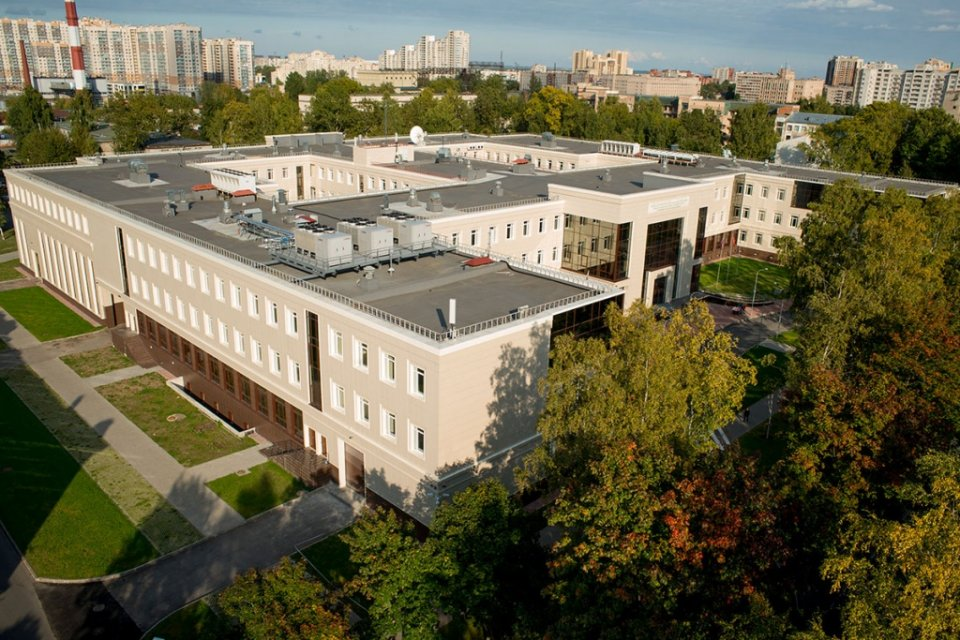
\includegraphics[keepaspectratio=true,scale=0.27] {my_folder/images/spbpu_new_bld_autumn}
	\captionof{figure}{Новый научно-исследовательский корпус СПбПУ \cite{spbpu-gallery} (с помощью окружения minipage)}\label{fig:spbpu-new-bld-autumn-minipage}  
	\vspace{\mfloatsep} % интервал  	
\end{minipage} % пример подключения minipage

\newpage


%% Вспомогательные команды - Additional commands
%
%\newpage % принудительное начало с новой страницы, использовать только в конце раздела
%\clearpage % осуществляется пакетом <<placeins>> в пределах секций
%\newpage\leavevmode\thispagestyle{empty}\newpage % 100 % начало новой страницы